\section{Problem 6}
\label{sec:problem6}

The LEO radius can be found from the altitude, and the GEO radius can be found from the fact that the period must be $24$~hours:
\begin{equation*}
r_1 = R_E + 300~\text{km} = 6678~\text{km}, \qquad
r_2 = \left(\frac{\mu \tau^2}{4\pi^2}\right)^{1/3}, \qquad
a = \frac{r_1+r_2}{2}
\end{equation*}
The circular speeds and the transfer orbit speeds at periapsis and apoapsis are
\begin{equation*}
v_{c1} = \sqrt{\frac{\mu}{r_1}}, \qquad
v_p = \sqrt{\frac{2\mu}{r_1}-\frac{\mu}{a}}, \qquad
v_a = \sqrt{\frac{2\mu}{r_2}-\frac{\mu}{a}}, \qquad
v_{c2} = \sqrt{\frac{\mu}{r_2}}
\end{equation*}
A fraction $f$ of the inclination change $\Delta i = 28.5^\circ$ is performed with the first impulse and $1-f$ with the second. Each impulse follows from Eq.~5.53:
\begin{equation*}
\Delta v_1(f) = \sqrt{v_{c1}^2 + v_p^2 - 2v_{c1}v_p\cos(f\,\Delta i)}, \qquad
\Delta v_2(f) = \sqrt{v_a^2 + v_{c2}^2 - 2v_a v_{c2}\cos\big((1-f)\,\Delta i\big)}
\end{equation*}
\begin{equation*}
\Delta V(f) = \Delta v_1(f) + \Delta v_2(f)
\end{equation*}

\subsection*{(a) and (b) Total impulse for $f=0$ and $f=1$}
All of the inclination change at apoapsis is $f=0$, and all of it at the initial LEO is $f=1$:
\begin{equation*}
\Delta V_{(a)} = \Delta V(0), \qquad \Delta V_{(b)} = \Delta V(1)
\end{equation*}
\subsection*{(c) Total impulse as a function of $f$}
$\Delta V(f)/v_{c1}$ for $f\in[0,1]$ in increments of $0.01$:

\begin{figure}[H]
\centering
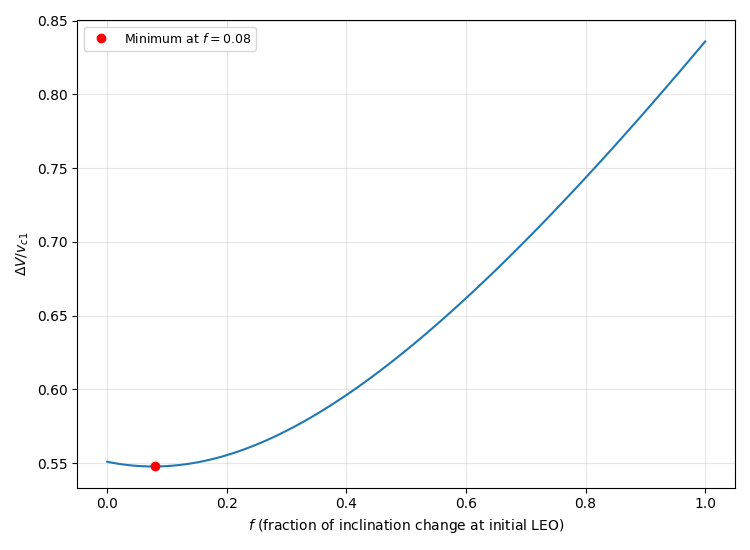
\includegraphics[width=0.65\textwidth]{problem6_dv_vs_f.png}
\caption{Normalized total impulse $\Delta V/v_{c1}$ vs.\ $f$.}
\label{fig:p6-dv}
\end{figure}

\subsection*{(d) Minimum-impulse fraction}
From \Cref{fig:p6-dv}, the smallest total impulse ($\Delta V/v_{c1} = 0.5478$) occurs at
\begin{equation*}
\boxed{f = 0.08}
\end{equation*}

\medskip
\noindent The expressions in parts (a) through (d) are evaluated in \texttt{problem6.py} with $\mu = 398600~\text{km}^3/\text{s}^2$ and $R_E = 6378$~km, giving:

\medskip
\programoutput{outputs/problem6.txt}

\FloatBarrier
